% !TeX spellcheck = en_GB 

\documentclass{tnreport}
%\documentclass[stage2a]{tnreport1} % If you are in 2nd year
%\documentclass[confidential]{tnreport1} % If you are writing confidential report

\def\reportTitle{Wordify} % Titre du mémoire
\def\reportAuthor{Ophélien Amsler \& Bertrand Müller}

\usepackage{lipsum}
\usepackage{subcaption}
\usepackage{adjustbox}
\usepackage{dirtree}
\usepackage{tikz}
\usepackage{multirow}
\usetikzlibrary{trees}
\usepackage{tikz-qtree}
\usepackage{makecell}
\usepackage{hhline}
\usepackage{colortbl}
\usepackage[most]{tcolorbox}
\usepackage{pdfpages}
\usepackage{draftwatermark}
\usepackage[stable]{footmisc}
\usepackage{hhline}
\usepackage{float}
\usepackage{graphicx}
\usepackage{enumitem}
\usepackage{wrapfig}

\usetikzlibrary{calc}
\usetikzlibrary{positioning}

\usepackage{listingsutf8}

\lstdefinelanguage{docker}{
  keywords={FROM, RUN, COPY, ADD, ENTRYPOINT, CMD,  ENV, ARG, WORKDIR, EXPOSE, LABEL, USER, VOLUME, STOPSIGNAL, ONBUILD, MAINTAINER},
  keywordstyle=\color{blue}\bfseries,
  identifierstyle=\color{black},
  sensitive=false,
  comment=[l]{\#},
  commentstyle=\color{purple}\ttfamily,
  stringstyle=\color{red}\ttfamily,
  morestring=[b]',
  morestring=[b]"
}

\lstdefinelanguage{docker-compose}{
  keywords={image, environment, ports, container_name, ports, volumes, links},
  keywordstyle=\color{blue}\bfseries,
  identifierstyle=\color{black},
  sensitive=false,
  comment=[l]{\#},
  commentstyle=\color{purple}\ttfamily,
  stringstyle=\color{red}\ttfamily,
  morestring=[b]',
  morestring=[b]"
}
\lstdefinelanguage{docker-compose-2}{
  keywords={version, volumes, services},
  keywordstyle=\color{blue}\bfseries,
  keywords=[2]{image, environment, ports, container_name, ports, links, build},
  keywordstyle=[2]\color{olive}\bfseries,
  identifierstyle=\color{black},
  sensitive=false,
  comment=[l]{\#},
  commentstyle=\color{purple}\ttfamily,
  stringstyle=\color{red}\ttfamily,
  morestring=[b]',
  morestring=[b]"
}

\lstset{basicstyle=\ttfamily,
  showstringspaces=false,
  commentstyle=\color{red},
  keywordstyle=\color{blue},
  inputencoding=utf8,
  extendedchars=true
}

\usepackage{listings}
\usepackage{xcolor}

\colorlet{punct}{red!60!black}
\definecolor{background}{HTML}{EEEEEE}
\definecolor{delim}{RGB}{20,105,176}
\colorlet{numb}{magenta!60!black}

\lstdefinelanguage{json}{
	basicstyle=\normalfont\ttfamily,
	numbers=left,
	numberstyle=\scriptsize,
	stepnumber=1,
	numbersep=8pt,
	showstringspaces=false,
	breaklines=true,
	frame=lines,
	backgroundcolor=\color{background},
	literate=
	*{0}{{{\color{numb}0}}}{1}
	{1}{{{\color{numb}1}}}{1}
	{2}{{{\color{numb}2}}}{1}
	{3}{{{\color{numb}3}}}{1}
	{4}{{{\color{numb}4}}}{1}
	{5}{{{\color{numb}5}}}{1}
	{6}{{{\color{numb}6}}}{1}
	{7}{{{\color{numb}7}}}{1}
	{8}{{{\color{numb}8}}}{1}
	{9}{{{\color{numb}9}}}{1}
	{:}{{{\color{punct}{:}}}}{1}
	{,}{{{\color{punct}{,}}}}{1}
	{\{}{{{\color{delim}{\{}}}}{1}
	{\}}{{{\color{delim}{\}}}}}{1}
	{[}{{{\color{delim}{[}}}}{1}
	{]}{{{\color{delim}{]}}}}{1},
}

\begin{document}

\maketitle

\cleardoublepage

\renewcommand{\baselinestretch}{0.5}\normalsize
\tableofcontents
\renewcommand{\baselinestretch}{1.0}\normalsize

\cleardoublepage

\chapter{Introduction}

In this report, we will introduce a new tool to improve our English skills while playing a game. The purpose of the project is to promote a new digital tool in order to learn English. Thus, our team worked on an innovative tool to enrich our vocabulary. For this project, the idea is to focus on the interactive side of the solution and to provide a non-existent tool. 

Why is this project relevant at the present time ? Nowadays, learning a language is a major challenge in an globalized society. English is one of the most widely spoken language in the world. It is an important mean for dialoguing and to be informed. However, the average English language level is uneven across different regions of the world and Europe. Our project is part of the desire to fill these gaps and to allow people to easily talk or to develop professionally. In addition, learning a new language can be tedious and time consuming. Our wish is to reduce this learning time for people having some knowledge in English. 

In order to present our game called \textbf{Wordify}, we decided to structure this report according to three different parts. The first one presents the game itself and its rules. In this first part, we want to provide a user documentation to know how to play and how the interface has to be used. The second is centered on a technical description of the game by presenting its architecture, the tools used, the difficulties encountered and the solutions found.

This report aims to present our new way of learning English and to highlight the needs in the current education system. 

\begin{center}
	
\includegraphics{figures/lets_play}
\end{center} 

\cleardoublepage

\chapter{Game}

This first part aims to describe the game principle and the platform used to play it. This section is deliberately non-technical to allow anyone to understand the concept and to know all the proposed features. 

\section{Principle}

In order to be in adequacy with this concept of interactivity, we made the choice to develop an online multiplayer game. The idea is to make a tool easily accessible by anyone, which allows to learn with friends. Overall, it is a cooperative game where the goal is to discover as many mystery words as possible. Is is therefore necessary to find sufficiently comprehensible hints to help a teammate, while making sure that they are not identical to those of the other players.

As previously mentioned, players will have to connect to a common online platform to collaborate and to guess as many words as possible. It is accessible from the following website address : \textbf{\textit{wordify.online}}. Once this page has been accessed from a browser (figure \ref{fig:wordify_home_page}), it is possible for a player to join a game or to create a new one. Then, he can invite his friends, his family members... The interface is intended to be original (retro effect) but simple to allow people to quickly understand how to start a new game. Once the player has joined a game, the rules, described in the next section, are applied. 

\bigskip

\begin{figure}[ht]
	\centering
	\fboxsep=1.2pt
	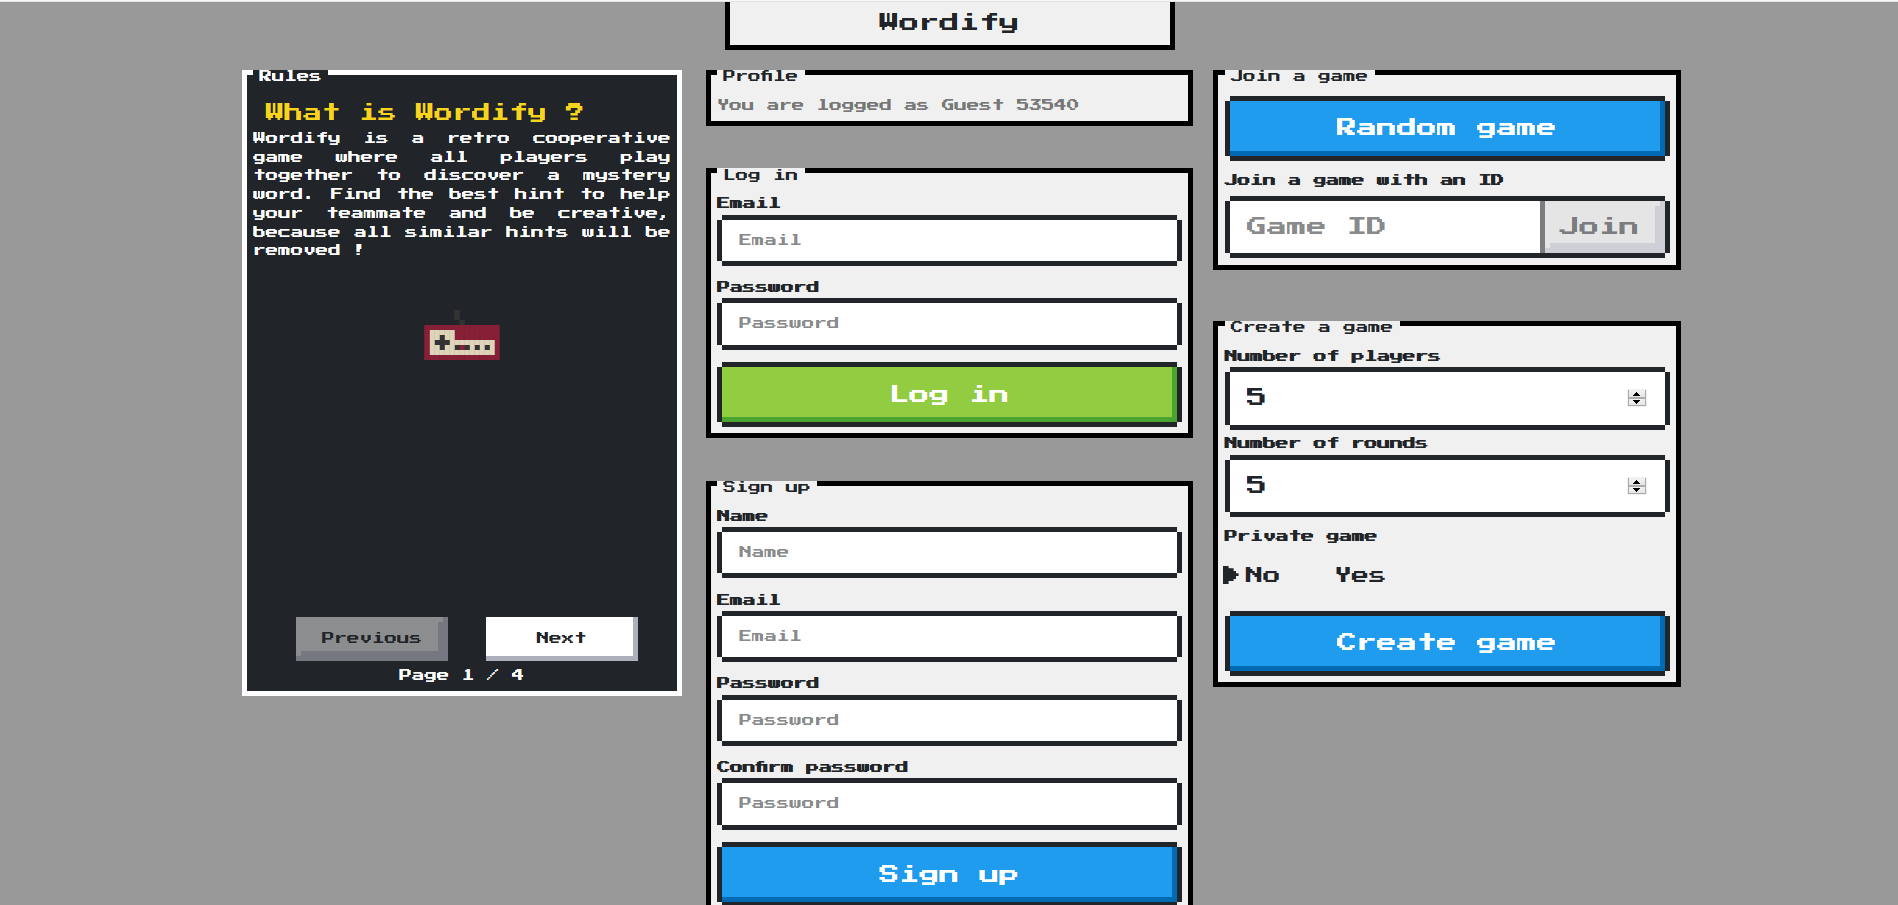
\includegraphics[scale=0.4]{figures/wordify_home_page}
	\caption{Wordify - Home page}
	\label{fig:wordify_home_page}
\end{figure} 

\clearpage

\section{Rules}

\label{chapter:rules}

\textbf{Number of players : 3 to 7}

Once the players are connected to a game, the first round will automatically be initialized with the designation of an active player. An active player is the player who will have to guess the word according to the hints proposed by his teammates. Once the player selection is made, the system selects a word among a list stored in the database. This action completes the initialization phase for the first round. 

The mystery word is then displayed to non-active players. Then, they have to write a word related to the word to be divined by the active player, by respecting the time limit. In parallel, they must be careful not to put obvious words that other players could write. So that the game to be interesting, it is important that players do not agree on the word they choose. If it is the case, the interest of the game is lost. 

When the words have been entered by the other players, they are displayed to the active player so that he can guess the initial word. Be careful, identical or similar words will be removed from the list of words displayed to the active player. That is why it is wise to find words from the semantic field referring to the word to be guessed. 

In the next round, a new player is designated as active. The same rules are applied for this new round. The game ends when the number of rounds, indicated at the game creation, have been completed. The goal is to get the maximum number of points, knowing that, if the active player finds the word, players win 1 point, but, in case of bad answer, the team looses 1 point and in case of non-proposal, it will not lose or win any point. 

A player can play games as many times as he wants. He can re-share the link of his new game to invite people he wants to play with. This game is fun and challenging !

\section{Educational aspect}

In order to foster English education, this game has an educational purpose. Indeed, its goal is to learn new words from other players and to improve our vocabulary. Moreover, it combines speed and reflection : this is therefore and effective way to reason quickly in English while having a good time. In this way, this game targets anyone wishing to improve their English level while avoiding long courses. It makes accessible the practice of English by providing a ludic way to learn it. 

In addition, such a game enables teachers to create contexts where English language is useful and meaningful. Even though games are often associated with entertainment, we do not have to forget their educational value, especially in teaching and learning foreign languages. Games are effective in the way that they create motivation, reduce student stress and enable language learners to communicate.

\cleardoublepage

\chapter{User documentation}

In this new part, we want to detail the user manual to know how to use the interface and to be able to play a game. In order to do that, we start with a brief presentation of the interface before continuing with the description of each proposed features. Like the previous section, this chapter has been written to be non-technical in order to make explanations accessible. 

\section{Interface}

Upon arrival on the platform, a player accesses the game homepage (figure \ref{fig:wordify_home_page}). As mentioned before, we decided to adopt a retro style to make it more attractive and to feel nostalgic about the first games developed on console. 

Apart from this design aspect, the player has access to different menus that will allow him to trigger specific actions. The figure \ref{fig:wordify_home_page_menus} shows the menus a player has access to.  The first one (\ref{fig:game_rules}) is used to present game rules. The second one (\ref{fig:login_form}) allows people to connect to their account and to have access to their statistics for the previously played rounds. The third one (\ref{fig:registration_form}) provides an access to a registration form to create a new account. The fourth menu (\ref{fig:random_game_2}) enables the player to join a random game with unknown people. Finally, the last one (\ref{fig:propose_word}) offers a way to propose new words to the game administrators, who can validate them and integrate them to the game. 

\begin{figure}[ht]
	\centering
	\fboxsep=1.2pt
	\begin{subfigure}[t]{0.3\textwidth}
		\centering
		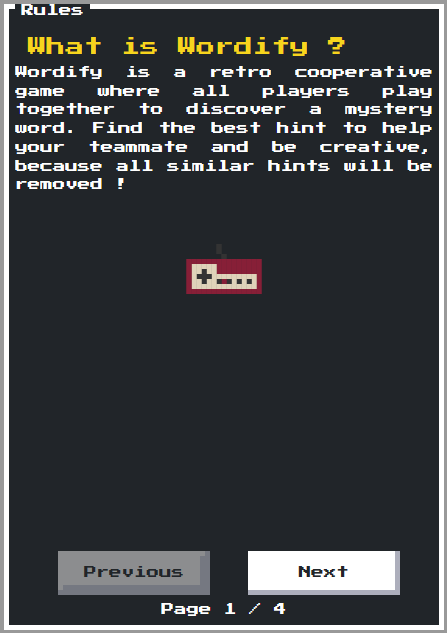
\includegraphics[height=1.2in]{figures/game_rules}
		\caption{Game rules}
		\label{fig:game_rules}
	\end{subfigure}
	\begin{subfigure}[t]{0.3\textwidth}
		\centering
		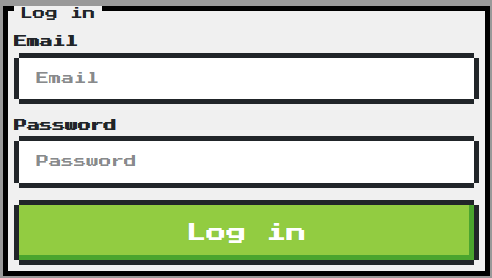
\includegraphics[height=1.2in]{figures/login_form}
		\caption{Login form}
		\label{fig:login_form}
	\end{subfigure}
	\begin{subfigure}[t]{0.3\textwidth}
		\centering
		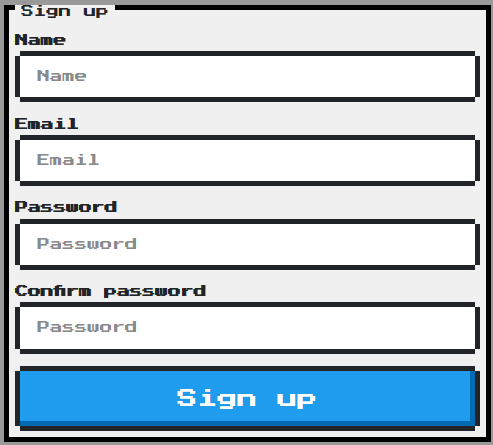
\includegraphics[height=1.2in]{figures/registration_form}
		\caption{Registration form}
		\label{fig:registration_form}
	\end{subfigure}
	\begin{subfigure}[t]{0.48\textwidth}
		\centering
		\vspace*{0.5cm}
		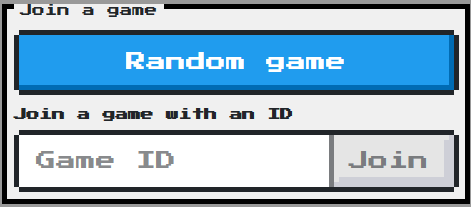
\includegraphics[height=0.9in]{figures/random_game}
		\caption{Random game}
		\label{fig:random_game_2}
	\end{subfigure}
	\begin{subfigure}[t]{0.48\textwidth}
		\centering
		\vspace*{0.5cm}
		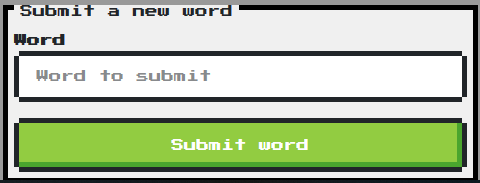
\includegraphics[height=0.9in]{figures/propose_word}
		\caption{Random game}
		\label{fig:propose_word}
	\end{subfigure}
	\caption{Wordify - Home page menus}
	\label{fig:wordify_home_page_menus}
\end{figure}

The game design is identical for all pages and allows players to easily interact with the application and to exploit all the associated features. 

\section{Functionalities}

\subsection{Player}

From now on, we want to detail the functionalities a player has access to while he is playing. This subpart can be considered as a typical scenario to play a game. 

\subsubsection{Join a game}

\begin{wrapfigure}{r}{0.4\linewidth}
	\centering
	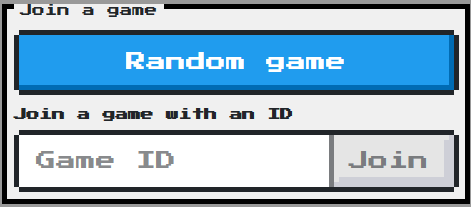
\includegraphics[scale=0.7]{figures/random_game}
	\caption{Join a game}
	\label{fig:join_game}
	\vspace*{-1cm}
\end{wrapfigure}

Of course, the interface offers a way to join a random game or a game previously created by a relative. The figure \ref{fig:join_game} shows the menu allowing to join a game. The player only have to click on the \textit{\textbf{Random Game}} button to perform this action. 

However, if the player does not want to join a random game, he can play with his friends or his family. He will have to copy the game's ID into the \textbf{\textit{Game ID}} field. The ID will be shared beforehand by the game creator. 

If he is logged in, he will be able to play with his account to update his stats. If it is not the case, a guest account will be automatically created to allow him to play. However, this time, game data will not be saved. 

Once the player managed to join a game, he is waiting for other players. The figure \ref{fig:waiting_players} shows the number of players currently connected, waiting to play the game. It is also possible to visualize the game ID in the upper left corner. It can be shared to anyone while the game is being initialized (waiting for players). 

\vspace*{0.1cm}

\begin{figure}[ht]
	\centering
	\fboxsep=1.2pt
	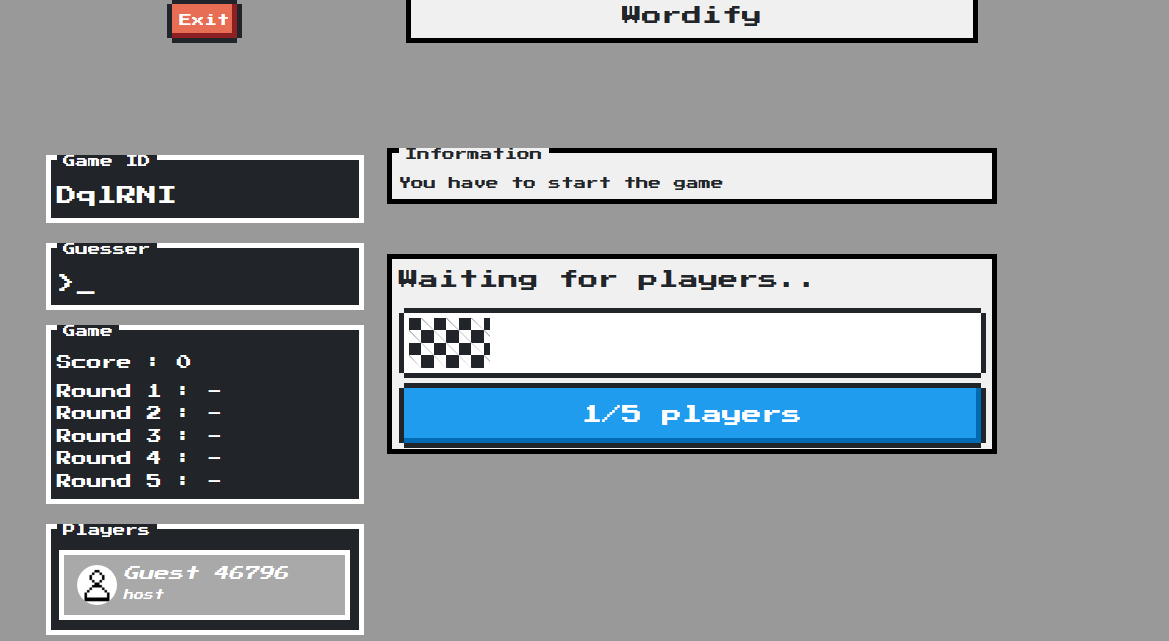
\includegraphics[scale=0.44]{figures/waiting_players}
	\caption{Waiting for players}
	\label{fig:waiting_players}
\end{figure} 

To start the game, the host will have to click on the blue button where the number of players is filled. All players present at the game launch will start to play. If not enough players are present, bots will be created. It is possible to identify them by the "robot" icon. 

\subsubsection{Enter a word}

\begin{wrapfigure}{r}{0.4\linewidth}
	\centering
	\vspace*{-0.2cm}
	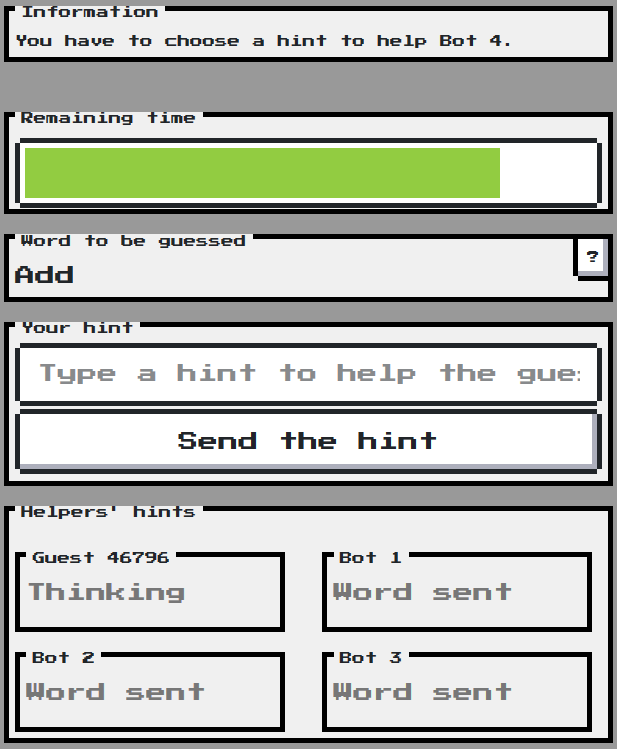
\includegraphics[scale=0.4]{figures/entering_word}
	\caption{Entering a word}
	\label{fig:entering_word}
\end{wrapfigure} 

When a player is not considered active, he has the responsibility to find a hint related to the word to be guessed by the active player. All non-active players perform the same task at the same time. They have a given time to enter a hint in the dedicated field (figure \ref{fig:entering_word}). If the time is up, no hint is sent and the person lost an additional chance to make the word to be guessed by the active player. 

Once each player has entered a hint, all non-active players see the words entered by the others. At this time, they must decide what words they want to keep by eliminating similar words. Once each player has voted, the scores are used to remove a word or not. The hints left are sent to the guesser. At this stage, we go to the next described functionality. 

\bigskip

\subsubsection{Guess a word}

\begin{wrapfigure}{r}{0.4\linewidth}
	\centering
	\vspace*{-0.5cm}
	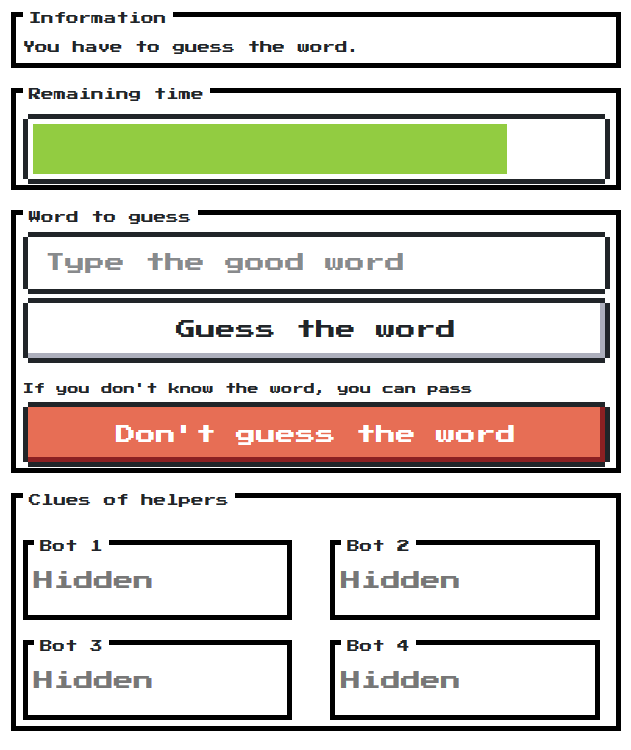
\includegraphics[scale=0.4]{figures/guessing_word}
	\caption{Guessing a word}
	\label{fig:guessing_word}
	\vspace*{-0.5cm}
\end{wrapfigure}

Once the game started, a player is designated to be the person to guess the word according to his teammates' hints. The active player must wait for the other players choose their hint, so that he can guess the sought word. The figure \ref{fig:guessing_word} shows the interface resulting from this waiting time. Once the hints have been displayed, he can try to guess the word in the allotted time or skip it (see the rules to know the number of points). 

Once the player has made his choice, the other players, waiting for his decision, know if their hint allowed him to find the right answer. The number of points earned is displayed in the interface and added to the total already obtained. At the end of the round, a new player is designated as the person to guess the next word.

\bigskip

\subsubsection{Chat}

\begin{wrapfigure}{r}{0.4\linewidth}
	\centering
	\vspace*{-2cm}
	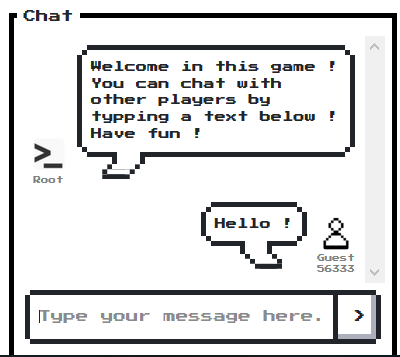
\includegraphics[scale=0.63]{figures/chat}
	\caption{Chat}
	\label{fig:chat}
	\vspace*{-2cm}
\end{wrapfigure}

Another feature we want to introduce is the ability to chat with other players sharing the same game. At the bottom right of the screen, it is possible to talk and to share feelings about the current game. The figure \ref{fig:chat} shows how the chat menu looks like.

\clearpage

\subsubsection{Get statistics}

\begin{wrapfigure}{r}{0.4\linewidth}
	\centering
	\vspace*{-2cm}
	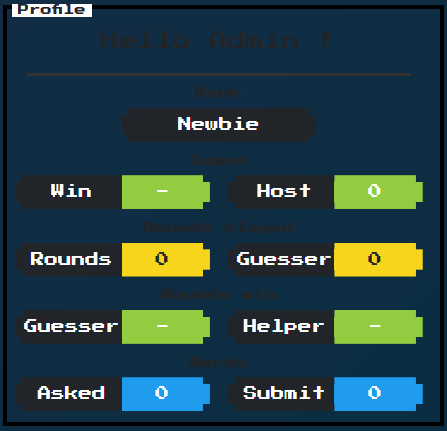
\includegraphics[scale=0.5]{figures/statistics}
	\caption{Statistics}
	\label{fig:statistics}
	\vspace*{-2cm}
\end{wrapfigure}

In addition to game-specific features, user has the possibility to access statistics about the previous played games. The figure \ref{fig:statistics} shows all the statistics a player has access to. They can be accessed from the home page if the player is connected with his own account. 

\bigskip
\bigskip
\bigskip

\subsubsection{Update profile}

\begin{wrapfigure}{r}{0.4\linewidth}
	\centering
	\vspace*{-2cm}
	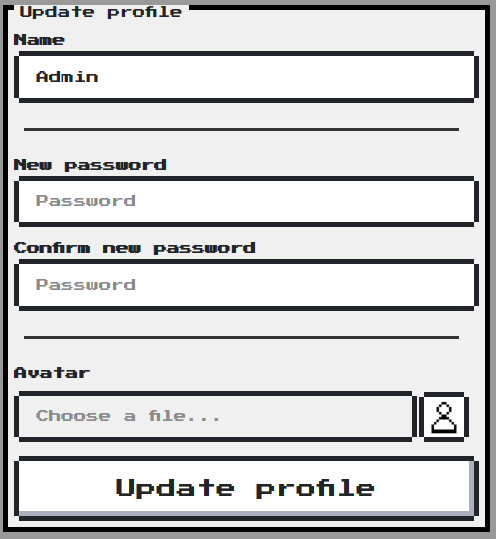
\includegraphics[scale=0.5]{figures/update_profile}
	\caption{Updating profile}
	\label{fig:update_profile}
	\vspace*{-3cm}
\end{wrapfigure}

Once the player is logged in, he can also update his pseudo, password and avatar. After the avatar has been changed, it is visible to the other players during a game. We wanted to offer the possibility to personalize his account. The figure \ref{fig:update_profile} shows the menu allowing to make these modifications. 

\bigskip
\bigskip

\subsubsection{Proposal of a new word}

\begin{wrapfigure}{r}{0.4\linewidth}
	\centering
	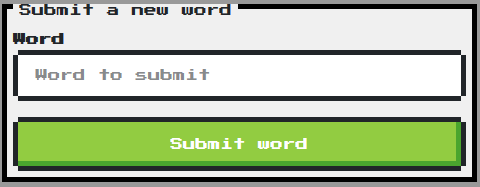
\includegraphics[scale=0.5]{figures/send_word}
	\caption{Sending a word}
	\label{fig:send_word}
\end{wrapfigure}

Finally, the last proposed feature is to propose a word to the game administrators. Once this word has been sent, an administrator will be able to include or not this word in the game. Then, it will be available for all games played after the validation was carried out. The figure \ref{fig:send_word} presents this menu allowing to indicate a word in the corresponding field. 

\subsection{Administrator}

To present all the proposed features, we have to place ourselves from an administrator responsibility point of view. In this part, we want to highlight the decisions that can be taken by this person in order to administer the game and to make it more enjoyable ! Of course, the administrator can be a player who has more important responsibilities. 

\subsubsection{Add a new word}

And administrator can add a new word so that it can be used in new games played by users. The figure \ref{fig:admin_add_word} shows the menu associated to this feature. 

\subsubsection{Validate a new word proposed by a player}

As mentioned above, a player may propose a new word to be added to the game. An administrator can access the proposed words and validate those he wants. The menu is shown in the figure \ref{fig:admin_validate_word}. 

\subsubsection{Delete a word}

Finally, he can also see a list of words that have already been validated by administrators. Thanks to this listing, he can decide to look at a word definition or to delete it if he deems it necessary. 

\bigskip

\begin{figure}[ht]
	\centering
	\begin{subfigure}[t]{0.5\textwidth}
		\centering
		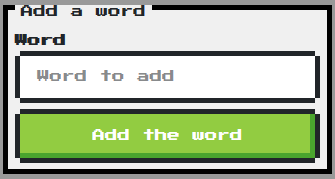
\includegraphics[height=1.5in]{figures/admin_add_word}
		\caption{Adding a word}
		\label{fig:admin_add_word}
	\end{subfigure}%
	~ 
	\begin{subfigure}[t]{0.5\textwidth}
		\centering
		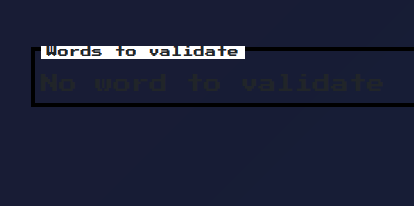
\includegraphics[height=1.5in]{figures/admin_validate_word}
		\caption{Validating a new word}
		\label{fig:admin_validate_word}
	\end{subfigure}
	\begin{subfigure}[t]{0.5\textwidth}
		\centering
		\vspace*{1cm}
		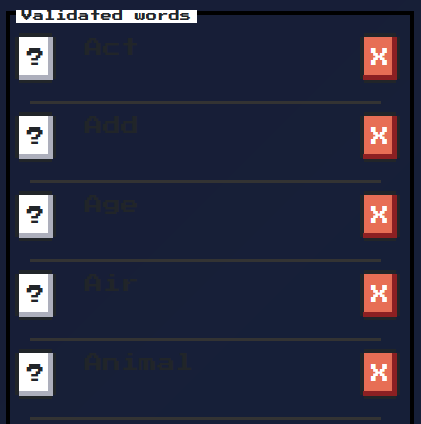
\includegraphics[scale=0.6]{figures/admin_validated_words}
		\caption{Validated words listing}
		\label{fig:admin_validated_words}
	\end{subfigure}
	\caption{Administrator functionalities}
\end{figure} 

\cleardoublepage

\chapter{Documentation technique}

Dans cette quatrième partie, on souhaite présenter la mise en oeuvre informatique de notre jeu en ligne. Pour cela, on a décidé de diviser ce chapitre en trois sous-parties : la partie non-visible par l'utilisateur (Back-End), la partie visible (Front-End) et la stratégie de déploiement adoptée pour que la solution soit accessible en ligne. Ces trois sous-parties sont ensuite compétées par la présentation de problèmes rencontrés et des solutions trouvées pour les résoudre. 

\section{Back-end}

\subsection{Laravel}

On souhaite donc débuter par la description de la partie serveur, c'est-à-dire à la partie non-visible par l'utilisateur. Pour structurer notre projet de la manière la plus efficace qui soit, nous avons fait le choix d'utiliser le framework Laravel qui s'appuie sur le patron de conception \textit{Modèle-Vue-Contrôleur} (MVC). En utilisant cet outil, actuellement très employé pour la création d'applications Web, nous avons pu utiliser quelques fonctionnalités déjà présentes pour nous concentrer principalement sur le développement du jeu en tant que tel. 

Ce framework repose sur le langage \textit{PHP} et offre notamment la possibilité de gérer les comptes utilisateurs. Il est alors possible de créer des comptes et de se connecter sans se préoccuper de la vérification des valeurs entrées (le framework gère efficacement la partie sécurité). Cependant, nous avons dû l'adapter pour intégrer ce type de système à notre jeu. Cela a demandé un travail d'intégration assez important pour être en mesure de lier les parties jouées à un compte utilisateur.

\subsection{Sockets}

\label{chapter:back_end_sockets}

Pour éviter des rechargements inopinés de page lorsqu'un jeu est en cours, nous avons veillé à utiliser des sockets. Cette technologie permet de communiquer avec le serveur sans avoir à recharger la page sur laquelle on se trouve, en vue de voir de potentiels changements s'afficher. Ceci garantit donc une navigation plus agréable pour l'utilisateur final sachant que le serveur est sensible à ses actions. 

Pour cela, nous avons dû utiliser des outils complémentaires et veiller à les associer au framework Laravel. Cette phase a constitué une partie importante de notre travail. En effet, nous avons dû configurer un outil appelé \textit{Redis} qui permet de sauvegarder les événements déclenchés par le serveur en réponse aux interactions faites par un ou plusieurs joueurs.

\subsection{API externe}

Par ailleurs, nous avons le choix d'utiliser une API externe pour récupérer des synonymes, des mots appartenant au même champ lexical ou des définitions de ces mots. Cet outil, appelé \textit{WordsAPI}, nous permet de constituer une base de données importante de mots afin de garantir un nombre conséquent de parties différentes. On évite ainsi aux joueurs de s'ennuyer et de recontrer fréquemment les mêmes mots. 

Pour l'employer de la manière le plus efficace qui soit, nous avons fait le choix de l'appeler depuis le serveur afin de stocker régulièrement les résultats de ces appels en base de données. Ainsi, après un certain nombre de parties jouées, on limite fortement le nombre d'appels effectués à ce service et on réduit le temps d'attente pour l'utilisateur. De cette manière, plus le nombre de parties jouées est important, plus l'expérience utilisateur est améliorée.

D'un point de vue des interfaces du jeu, un joueur ou un administrateur peut ainsi obtenir une définition d'un mot qu'il ne connaît pas (ceci enrichit donc leur vocabulaire) et les robots, jouant à la place de vrais joueurs, peuvent trouver des mots du même champ lexical que celui du mot à faire deviner. 

\subsection{PostgreSQL}

Enfin, sur le serveur, nous utilisons un dernier outil qui s'appelle \textit{PostgreSQL}. Ce dernier correspond à une base de données permettant de stocker toutes les informations quant au bon déroulement du jeu. Ainsi, on peut retrouver tous les comptes utilisateurs créés, tous les mots déjà enregistrés, les statistiques sur un joueur etc... 

L'idée ici est de persister les données essentielles pour le jeu. Par exemple, on évite ainsi de demander aux utilisateurs de créer un compte à chaque fois qu'il souhaite jouer. De plus, \textit{PostgreSQL} est un outil fiable et s'utilise parfaitement avec le framework \textit{Laravel}. 

\section{Front-End}

\subsection{Langages de programmation}

Concernant la partie visible par l'utilisateur, nous avons dû utiliser les standards du Web pour que le jeu soit affichable dans un navigateur. Ainsi, le premier d'entre eux est le langage \textit{Hypertext Markup Language} (HTML). Il offre un moyen d'afficher le contenu d'une page Web tel que du texte et des images. Il permet simplement de créer les éléments liés au contenu.

Ce langage est complété par l'utilisation d'un second langage appelé \textit{Cascading Style Sheets} (CSS) qui vise à mettre en forme le contenu d'une page. Cette mise en page est réalisée par la définition de règles propres au langage (style des titres, taille d'écriture, couleurs...). En réalité, le style s'applique sur les balises définies grâce au langage \textit{HTML}. 

Enfin, il est nécessaire de pouvoir modifier le contenu d'une page dynamiquement, c'est-à-dire sans avoir à recharger la page. Le langage \textit{JavaScript} (JS) répond à ce besoin en permettant notamment de gérer les interactions et les animations sur une page. Il est donc beaucoup plus évolué que le \textit{HTML} et le \textit{CSS}.

\subsection{Design}

\urlstyle{sf}

Comme évoqué dans la première partie de ce rapport, nous avons fait le choix d'adopter un style rétro pour notre jeu. Pour cela, le framework utilisé s'appelle \textit{NES.css}. Grâce à cet outil, il est possible de créer des effets de pixélisation sur les éléments présents. La page \url{https://nostalgic-css.github.io/NES.css/} regroupe tous les éléments pouvant être utilisés pour notre jeu. 

\subsection{Sockets}

Comme dans la partie \ref{chapter:back_end_sockets}, il est nécessaire de gérer les sockets mais du côté utilisateur. Afin de pouvoir être sensible aux événements déclenchés par le serveur, le client doit pouvoir les détecter et réaliser des modifications en conséquence sur la page courante. La librairie \textit{JavaScript} utilisée s'appelle \textit{EchoJS} et nécessite simplement d'être incluse dans le contenu de la page. Afin de mieux comprendre son fonctionnement, il est possible de se reporter au schéma d'architecture dans la partie \ref{chapter:global_architecture}.

\section{Déploiement}

\subsection{Docker}

Cette sous-partie s'attache à décrire la stratégie de déploiement adoptée. Afin de garantir un déploiement efficace et de partager un environnement de travail commun, nous avons décidé d'utiliser la technologie \textit{Docker}. Il s'agit d'un outil basé sur la conteneurisation permettant le déploiement automatique de services selon une configuration définie par les développeurs. Nous avons donc dû réaliser cette configuration en nous basant sur nos connaissances quant à cet outil et à la documentation fournie pour le framework Laravel. L'annexe \ref{annexe:docker_compose} montre le fichier \textit{docker-compose.yml} utilisé pour créer nos conteneurs, c'est-à-dire nos services utiles au bon déroulement du jeu.

Pourquoi avons-nous décidé de réaliser cette configuration ? En réalité, l'utilisation de Docker est une force puisqu'il permet de déployer l'application sur n'importe quel serveur où docker est installé. Nous avons donc voulu rendre l'application durable dans le temps et installable sur n'importe quel système.

\subsection{Nom de domaine}

Afin de rendre accessible notre plateforme à n'importe quelle personne, nous avons choisi d'acheter un nom de domaine pour que le jeu puisse être en ligne. Le nom de domaine choisi est lié au nom de notre jeu (Wordify), à savoir : \textbf{\textit{wordify.online}}.

Pour que le nom de domaine redirige vers notre jeu, nous avons dû configurer le \textit{Domain Name Server} (DNS) de notre serveur. Une fois cette configuration réalisée, il est alors possible de lancer une partie en multijoueur avec des personnes se trouvant potentiellement dans différentes parties du monde. Le jeu est alors lancé selon les règles exposées dans la partie \ref{chapter:rules}. 

\section{Architecture globale}

\label{chapter:global_architecture}

\begin{figure}[ht]
	\centering
	\fboxsep=1.2pt
	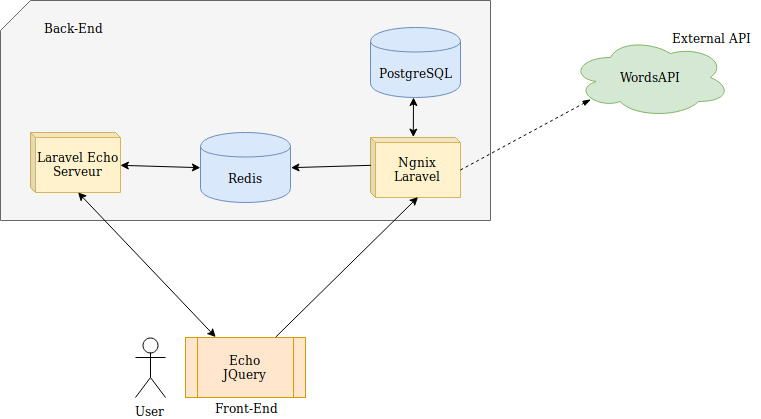
\includegraphics[scale=0.6]{figures/diagram}
	\caption{Diagramme d'architecture}
	\label{fig:achitecture_diagram}
\end{figure} 

\section{Problèmes rencontrés}

\subsection{Gestion d'un salon de jeu}

Pour choisir le joueur actif, le serveur a besoin de connaître l'ensemble des joueurs afin de limiter le nombre de joueurs dans chaque partie et d'ajouter le bon nombre de robots. Ce système est difficile à mettre en oeuvre car le serveur ne peut pas connaître les utilisateurs présents dans le salon en temps réel. Lorsqu'un utilisateur se connecte, il doit faire une demande au serveur. Nous pouvons donc savoir le nombre d'utilisateurs entrants. Cependant, si un utilisateur se déconnecte, aucun événement ne sera déclenché côté serveur. Seuls les utilisateurs présents dans le salon sont informés grâce à la librairie \textit{EchoJS}.

\subsection{Solutions adoptées}

\subsubsection{Envoi du départ d'un joueur par le joueur hôte}

Avec cette solution, à chaque fois qu'un joueur se déconnectait, l'hôte notifiait le serveur pour lui indiquer le départ du joueur. Cependant, si un joueur reactualisait la page, l'hôte envoyait son départ de façon asynchrone. Il arrivait que le joueur soit revenu dans la partie avant que le serveur ait reçu une notification quant à son départ. De ce fait, le joueur était dans la partie mais le serveur le considérait comme absent.

Autre problème de cette solution : lorsque l'hôte quittait la partie, il était difficile d'en désigner un nouveau.

Suite à ces difficultés, nous avons donc cherché une autre solution.

\subsubsection{Utilisation de l'API Laravel Echo Serveur}

Une autre solution est l'utilisation de l'API \textit{Laravel Echo Serveur}. En effet, celle-ci peut nous permettre de connaître la liste des joueurs présents dans un salon de jeu. Pour permettre l'affichage des joueurs en ligne, le front utilisera les événements reçus depuis \textit{EchoJS}. Pour créer les parties et savoir s'il reste de place dans une partie, le serveur appellera l'API \textit{Laravel Echo Serveur}.

Avec cette solution, lorsque l'hôte quitte la partie, chaque joueur demande au serveur de désigner le nouvel hôte. Grâce à l'API \textit{Laravel Echo Serveur}, le serveur peut vérifier si l'hôte a bien quitté la partie. Si tel est le cas, il choisit aléatoirement un utilisateur et transmet le nouvel hôte à tous les joueurs en ligne.\\

\cleardoublepage

\chapter{Conclusion}

To finalize this report, wa want to conclude about our project and the developments we did. As for our initial goal, namely the realization of a multiplayer online game, we managed to achieve it while learning new technologies. More specifically, we managed to develop an educational game to facilitate English learning while having a good time. In order to learn new words, it is possible to join a game and to search for synonyms according to the searched word. We are therefore proud to make the English language accessible to anyone, by using a simple computer with a browser. 

However, improvements could be planned for future application versions in order to improve the user experience. We have listed improvements we foresee for the future :

\begin{itemize}
	\item \underline{Improve usability.} Although the game is rather good from this point of view, we can however consider improving the user experience by repositioning some menus on each page. Moreover, it could make the application more accessible to a younger audience (primary school). 
	
	\item \underline{Add difficulty levels.} To make the game more attractive and more challenging, we can imagine to create difficulty levels when playing with robots. Consequently, we would have more or less complicated synonyms to understand. 
	
	\item \underline{Forgotten password request.} A minor but important feature is to provide the user a way to change his password by indicating he has forgotten it. It will be necessary to install a system to send automatically emails to change the password, thanks to a link usable via a browser. 
	
	\item \underline{Test the application with different socio-professional categories.} To have opinions on the first version of the application, we could organize test sessions. These tests could allow us to know if the user experience is optimal. 
	
	\item \underline{Propose the application to primary schools.} After having tested the application with children, it could be interesting to approach primary schools if tests are successful. The game could be an educational tool for learning languages from an early age. Moreover, this fits with governments' desire to develop access to digital tools. 
	
	\item \underline{Suggest other languages to play with.} In the same way, if the tests are successful, we can include other languages to facilitate their learning. 
	
	\item \underline{Promote the application.} Finally, the application has a real success, we could promote it on various social networks or platforms to make it popular. 
\end{itemize}

\cleardoublepage

\begin{otherlanguage}{british}
\listoffigures

\cleardoublepage

\appendix
\part*{Annexes}
\addcontentsline{toc}{part}{Annexes}
\end{otherlanguage}

\cleardoublepage

\chapter{Technologies}

\section{Back-End}
\textbf{Laravel} : https://laravel.com/\\
\textbf{Laravel Echo Server} : https://github.com/tlaverdure/laravel-echo-server\\
\textbf{PostgreSQL} : https://www.postgresql.org/\\
\textbf{Redis} : https://redis.io/\\

\section{Front-End}
\textbf{Nes CSS} : https://nostalgic-css.github.io/NES.css/\\
\textbf{HTML} : https://fr.wikipedia.org/wiki/Hypertext \_Markup \_Language\\
\textbf{JavaScript} : https://fr.wikipedia.org/wiki/JavaScript\\
\textbf{JQuery} : https://jquery.com/\\
\textbf{Bootstrap} : https://getbootstrap.com/\\
\textbf{Laravel Echo} : https://github.com/laravel/echo\\

\section{External API}
\textbf{WordsApi} : https://www.wordsapi.com/\\

\section{Deployment}
\textbf{Docker} : https://www.docker.com/\\


\cleardoublepage

\chapter{Homepage}
\vspace{-1.5cm}
\begin{center}
	\rotatebox{90}{
		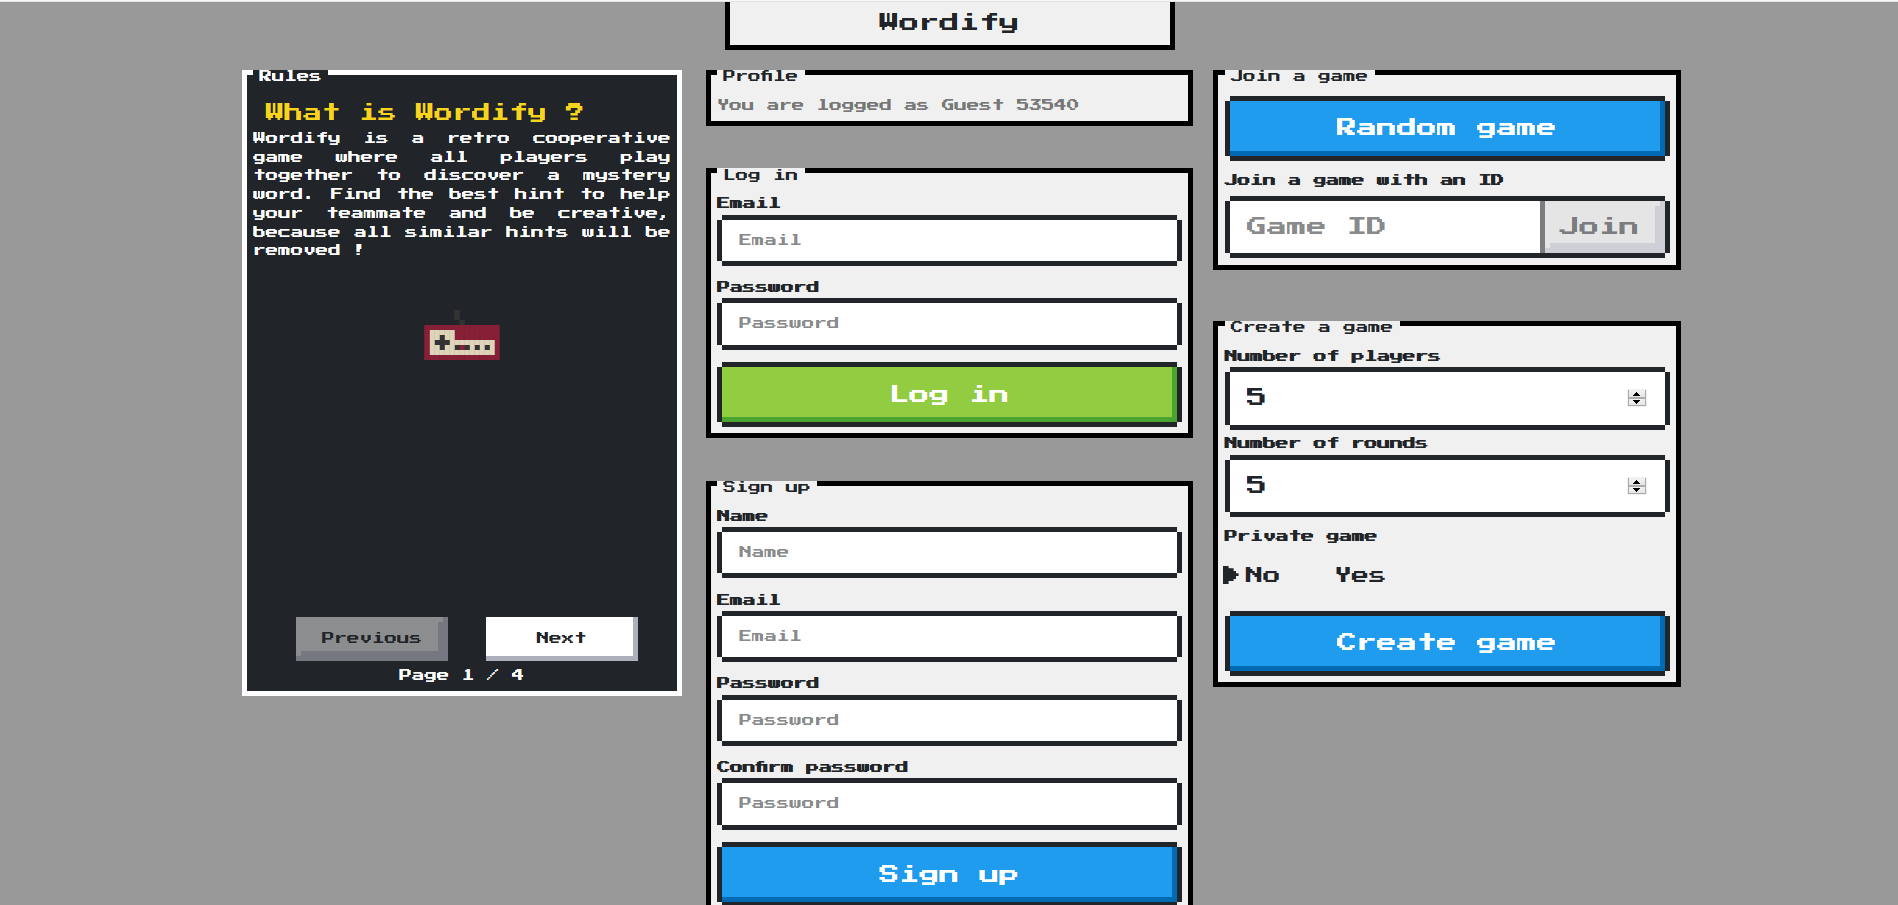
\includegraphics[scale=0.52]{figures/wordify_home_page}
	}
\end{center}

\cleardoublepage

\chapter{Waiting players page}
\vspace{-1.5cm}
\begin{center}
	\rotatebox{90}{
		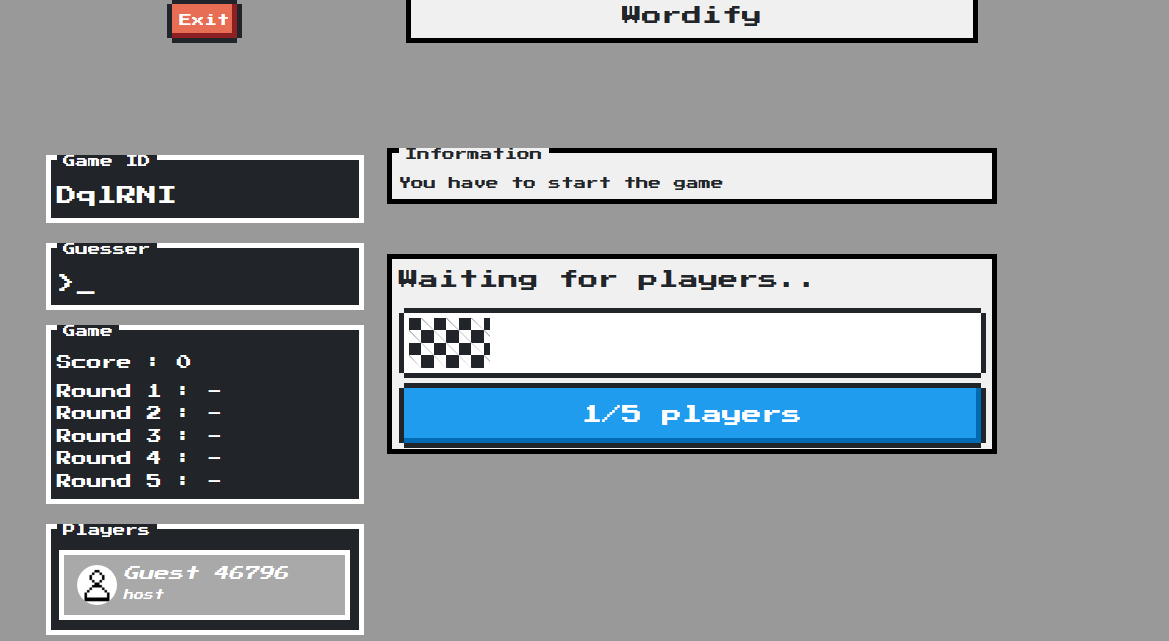
\includegraphics[scale=0.85]{figures/waiting_players}
	}
\end{center}

\cleardoublepage

\chapter{Game page}
\vspace{-1.5cm}
\begin{center}
	\rotatebox{90}{
		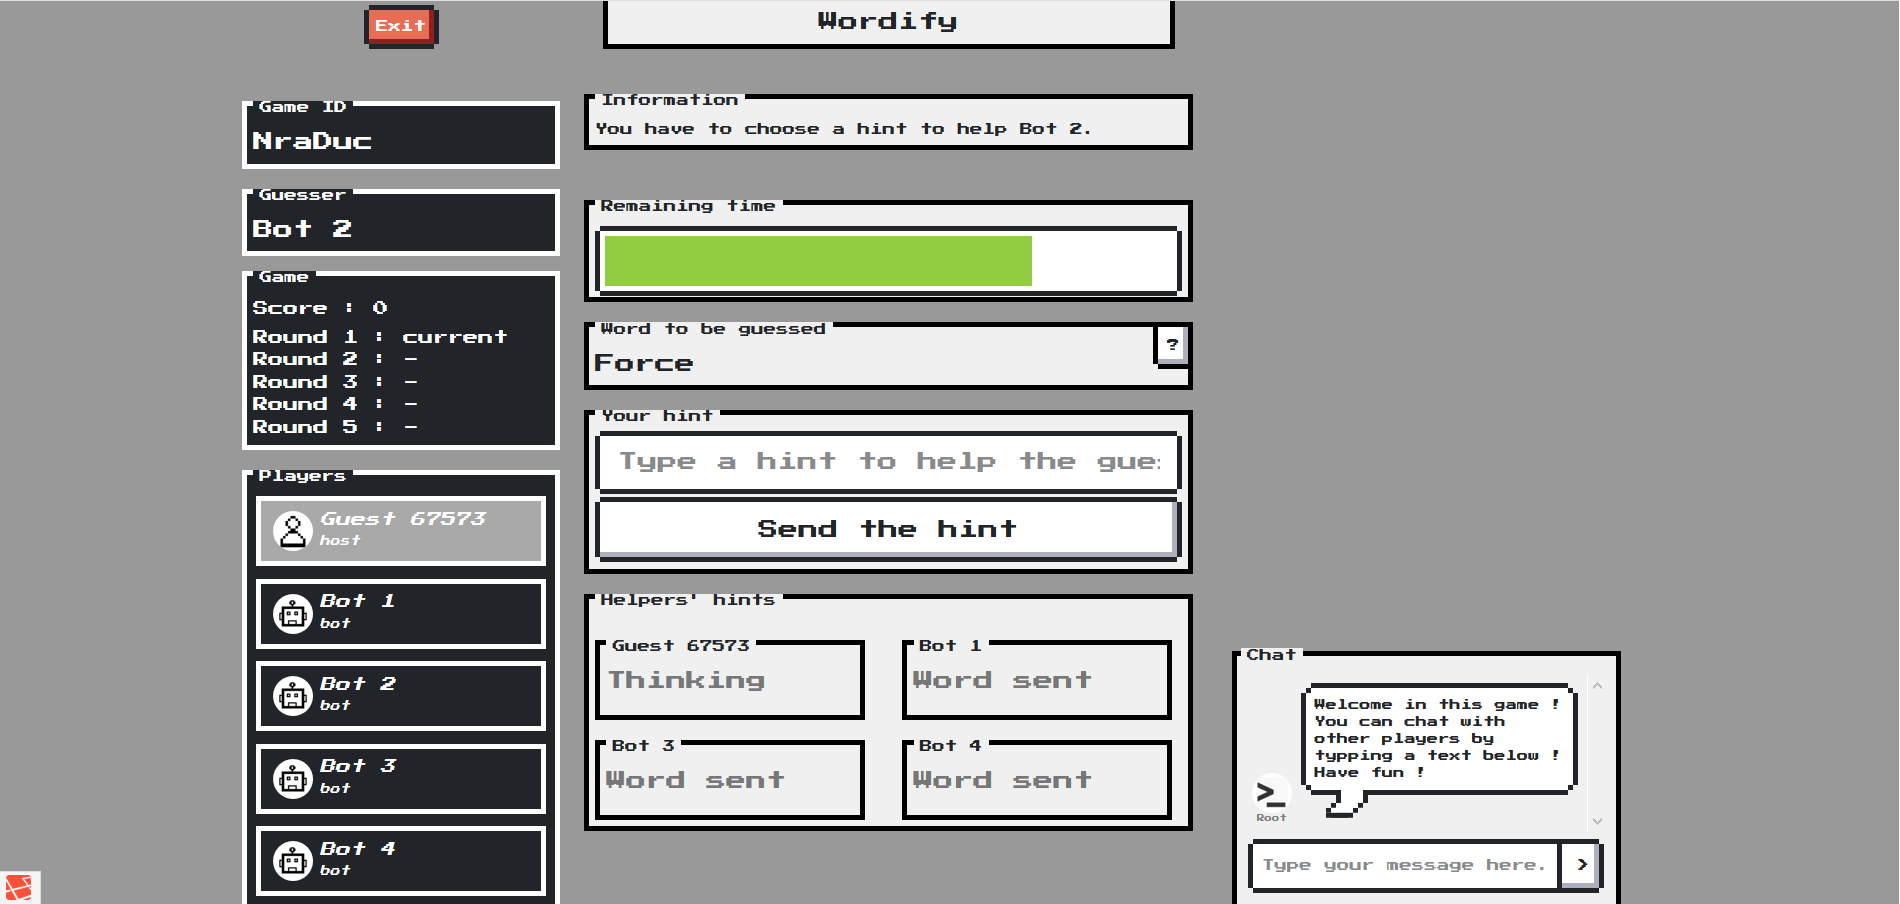
\includegraphics[scale=0.52]{figures/game_page}
	}
\end{center}

\cleardoublepage

\chapter{Back-End - Docker Configuration}
\label{annexe:docker_compose}
\vspace{0.5cm}
\begin{center}
	\vspace*{-0.8in}
	\lstinputlisting[language=docker-compose-2,basicstyle=\footnotesize]{../docker-compose.yml}
\end{center}

\cleardoublepage

\chapter{Front-End - JSON file}
\label{annexe:game_json}
\vspace{0.5cm}
\begin{center}
	\vspace*{-0.8in}
	\lstinputlisting[language=json,basicstyle=\footnotesize]{figures/game.json}
\end{center}

\end{document}
